%
% This is a borrowed LaTeX template file for lecture notes for CS267,
% Applications of Parallel Computing, UCBerkeley EECS Department.
% Now being used for CMU's 10725 Fall 2012 Optimization course
% taught by Geoff Gordon and Ryan Tibshirani.  When preparing 
% LaTeX notes for this class, please use this template.
%
% To familiarize yourself with this template, the body contains
% some examples of its use.  Look them over.  Then you can
% run LaTeX on this file.  After you have LaTeXed this file then
% you can look over the result either by printing it out with
% dvips or using xdvi. "pdflatex template.tex" should also work.
%

\documentclass[twoside]{article}
\setlength{\oddsidemargin}{0.25 in}
\setlength{\evensidemargin}{-0.25 in}
\setlength{\topmargin}{-0.6 in}
\setlength{\textwidth}{6.5 in}
\setlength{\textheight}{8.5 in}
\setlength{\headsep}{0.75 in}
\setlength{\parindent}{0 in}
\setlength{\parskip}{0.1 in}

%
% ADD PACKAGES here:
%

\usepackage{amsmath,amsfonts,graphicx}

%
% The following commands set up the lecnum (lecture number)
% counter and make various numbering schemes work relative
% to the lecture number.
%
\newcounter{lecnum}
\renewcommand{\thepage}{\thelecnum-\arabic{page}}
\renewcommand{\thesection}{\thelecnum.\arabic{section}}
\renewcommand{\theequation}{\thelecnum.\arabic{equation}}
\renewcommand{\thefigure}{\thelecnum.\arabic{figure}}
\renewcommand{\thetable}{\thelecnum.\arabic{table}}

%
% The following macro is used to generate the header.
%
\newcommand{\lecture}[4]{
   \pagestyle{myheadings}
   \thispagestyle{plain}
   \newpage
   \setcounter{lecnum}{#1}
   \setcounter{page}{1}
   \noindent
   \begin{center}
   \framebox{
      \vbox{\vspace{2mm}
    \hbox to 6.28in { {\bf EE302 - Feedback Systems
	\hfill Spring 2019} }
       \vspace{4mm}
       \hbox to 6.28in { {\Large \hfill Lecture #1 \hfill} }
       \vspace{2mm}
       \hbox to 6.28in { {\it Lecturer: #2 \hfill } }
      \vspace{2mm}}
   }
   \end{center}
   \markboth{Lecture #1}{Lecture #1}

   \vspace*{4mm}
}
%
% Convention for citations is authors' initials followed by the year.
% For example, to cite a paper by Leighton and Maggs you would type
% \cite{LM89}, and to cite a paper by Strassen you would type \cite{S69}.
% (To avoid bibliography problems, for now we redefine the \cite command.)
% Also commands that create a suitable format for the reference list.
\renewcommand{\cite}[1]{[#1]}
\def\beginrefs{\begin{list}%
        {[\arabic{equation}]}{\usecounter{equation}
         \setlength{\leftmargin}{2.0truecm}\setlength{\labelsep}{0.4truecm}%
         \setlength{\labelwidth}{1.6truecm}}}
\def\endrefs{\end{list}}
\def\bibentry#1{\item[\hbox{[#1]}]}

%Use this command for a figure; it puts a figure in wherever you want it.
%usage: \fig{NUMBER}{SPACE-IN-INCHES}{CAPTION}
\newcommand{\fig}[3]{
			\vspace{#2}
			\begin{center}
			Figure \thelecnum.#1:~#3
			\end{center}
	}
% Use these for theorems, lemmas, proofs, etc.
\newtheorem{theorem}{Theorem}[lecnum]
\newtheorem{lemma}[theorem]{Lemma}
\newtheorem{proposition}[theorem]{Proposition}
\newtheorem{claim}[theorem]{Claim}
\newtheorem{corollary}[theorem]{Corollary}
\newtheorem{definition}[theorem]{Definition}
\newenvironment{proof}{{\bf Proof:}}{\hfill\rule{2mm}{2mm}}

% **** IF YOU WANT TO DEFINE ADDITIONAL MACROS FOR YOURSELF, PUT THEM HERE:

\begin{document}

% Lecture Details
\lecture{8}{Asst. Prof. M. Mert Ankarali}

\par 

\section{Second Order Systems}

Let's derive the transfer functions for the following electrical and
mechanical systems

    \begin{minipage}[h]{1\linewidth}
    \begin{center}
     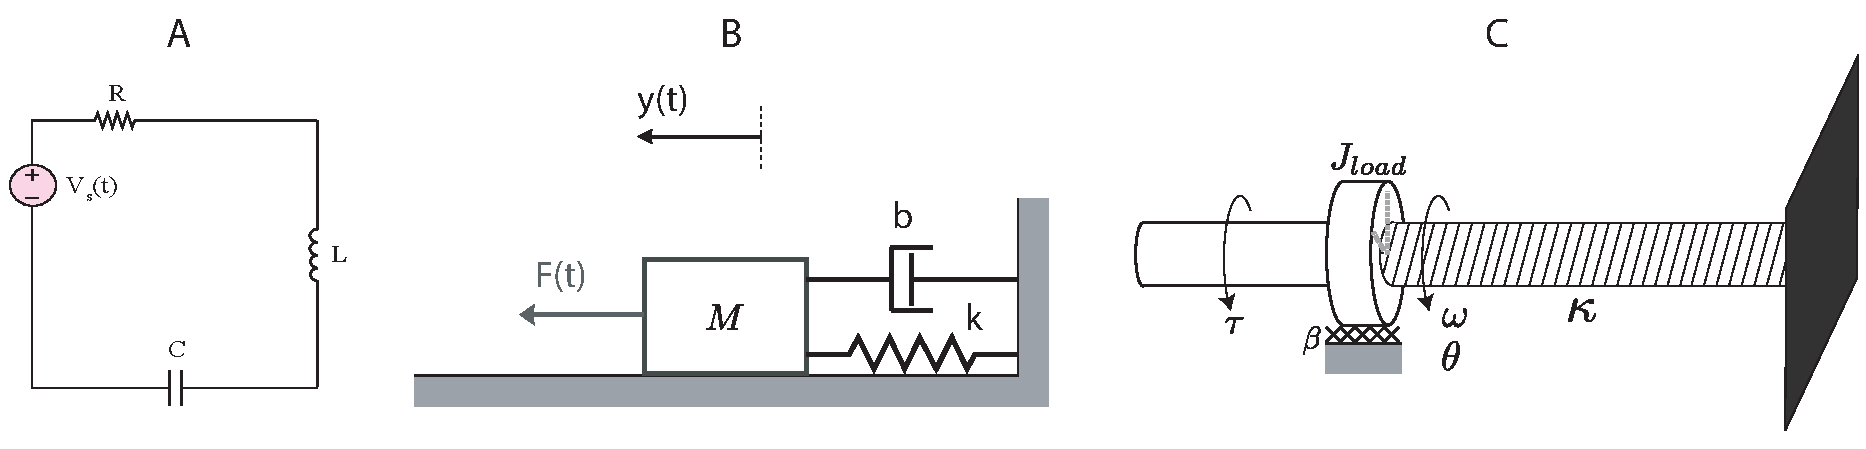
\includegraphics[width=1\textwidth]{2ndOrderSystems}
    \end{center}
  \end{minipage}

\begin{align*}
  G_A(s) &= \frac{V_C(s)}{V_s(s)} = \frac{\frac{1}{LC}}{s^2 +
  \frac{R}{L} s + \frac{1}{LC} }
\\ 
  G_B(s) &= \frac{Y(s)}{F(s)} = \frac{\frac{1}{M}}{s^2 +
  \frac{b}{M} s + \frac{k}{M} }
\\
   G_C(s) &= \frac{\Theta(s)}{\mathcal{T}(s)} = \frac{\frac{1}{J}}{s^2 +
  \frac{\beta}{J} s + \frac{\kappa}{J} }
\end{align*}

Most of the (passive) second order systems, can be put into the following the
standard form
%
\begin{align*}
G(s) =  K_{DC} \frac{\omega_n^2}{s^2 + 2 \zeta \omega_n s + \omega_n} 
\end{align*}
%
where

 \begin{minipage}[h]{1\linewidth}
\begin{tabular}{|c|l|}
\hline
 $0 < \omega_n$ & Undamped natural frequency
 \\
 $0 < \zeta $ & Damping ratio
 \\
 $K_{DC}$ & DC Gain
\\
\hline
\end{tabular}
  \end{minipage}

\vspace{12pt}

Accordingly for the systems that we analyzed previously we have the
following relations
%
\begin{align*}
A:& \quad  \omega_n = \sqrt{\frac{1}{LC}} \ , \ \zeta = \frac{R}{2}
  \sqrt{ \frac{C}{L} } \ , \ K_{DC} = 1
\\
B:& \quad  \omega_n = \sqrt{\frac{k}{M}} \ , \ \zeta = \frac{b}{2}
  \sqrt{ \frac{1}{M k} } \ , \ K_{DC} = \frac{1}{k}
\\
C:& \quad  \omega_n = \sqrt{\frac{\kappa}{J}} \ , \ \zeta = \frac{b}{2}
  \sqrt{ \frac{1}{J \kappa} } \ , \ K_{DC} = \frac{1}{\kappa}
\end{align*}

\textbf{Definition:} Given a transfer function, $G(s) =
\frac{N(s)}{D(s)}$, where $N(s)$ and $D(s)$ are polynomials in $s$.
Roots of $N(s)$ are called ``zeros'' of $G(s)$, and roots of $D(s)$
are called the ``poles'' of $G(s)$. 

Behavior of the output $y(t)$ are majorly determined by the pole
locations. 

\subsection{Step Response Types for the Second Order System in Standard
  Form}

Given that $G(s) = \frac{\omega_n^2}{s^2 + 2 \zeta \omega_n s +
  \omega_n^2}$, the poles can be computed as
%
\begin{align*}
  s_{1,2} = - \zeta \omega_n \pm \omega_n \sqrt{\zeta^2 - 1}
\end{align*}

\textbf{Case 1:} When $\zeta = 0$, the system becomes undamped and
$G(s)$ takes the form
%
\begin{align*}
  G(s) = \frac{\omega_n^2}{s^2 + \omega_n^2}
\end{align*}
%
We can compute the step-response as
%
\begin{align*}
 Y(s) &= G(s) U(s) = \frac{1}{s} \frac{\omega_n^2}{s^2 + \omega_n^2} =
        \frac{1}{s} - \frac{s}{s^2 + \omega_n^2}
\\
y(t) &= 1 - \cos(\omega_n t) \quad \mathrm{for} \ t > 0 
\end{align*}
%
Pole locations and step response when $\zeta = 0$ (undamped), is illustrated in
the Figure below

    \begin{minipage}[h]{1\linewidth}
    \begin{center}
     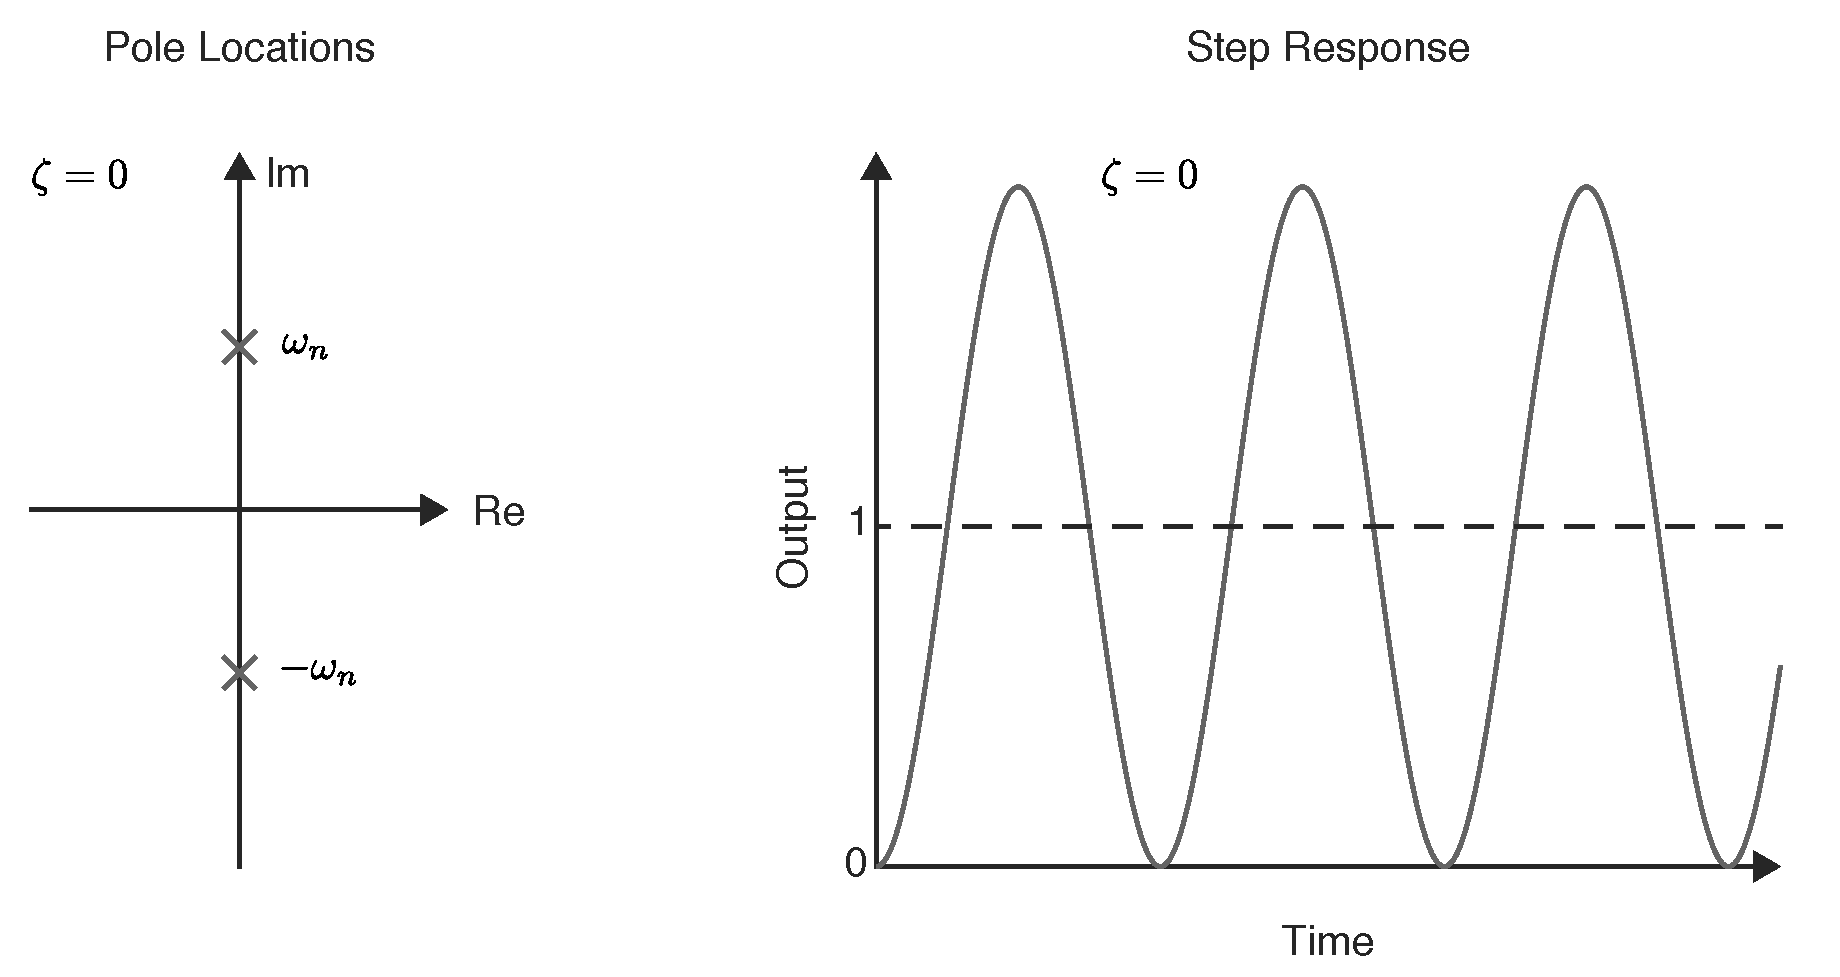
\includegraphics[width=0.7\textwidth]{undamped}
    \end{center}
  \end{minipage}

\textbf{Case 2:} When $\zeta = 1$, the system becomes ``critically'' damped and
$G(s)$ takes the form
%
\begin{align*}
	G(s) = \frac{\omega_n^2}{s^2 + 2 \omega_n s + \omega_n} = \frac{\omega_n^2}{(s + \omega_n )^2}  
\end{align*}
%
We can compute the step-response as
%
\begin{align*}
 Y(s) &= G(s) U(s) = \frac{1}{s} \frac{\omega_n^2}{(s + \omega_n )^2}  
 = \frac{1}{s} -  \frac{1}{s + \omega_n} + \frac{\omega_n}{(s + \omega_n)^2} 
\\
y(t) &= 1 - e^{-\omega_n t} - \omega_n t e^{-\omega_n t}
\end{align*}
%
Pole locations and step response when $\zeta = 1$ (critically damped), is illustrated in
the Figure below

    \begin{minipage}[h]{1\linewidth}
    \begin{center}
     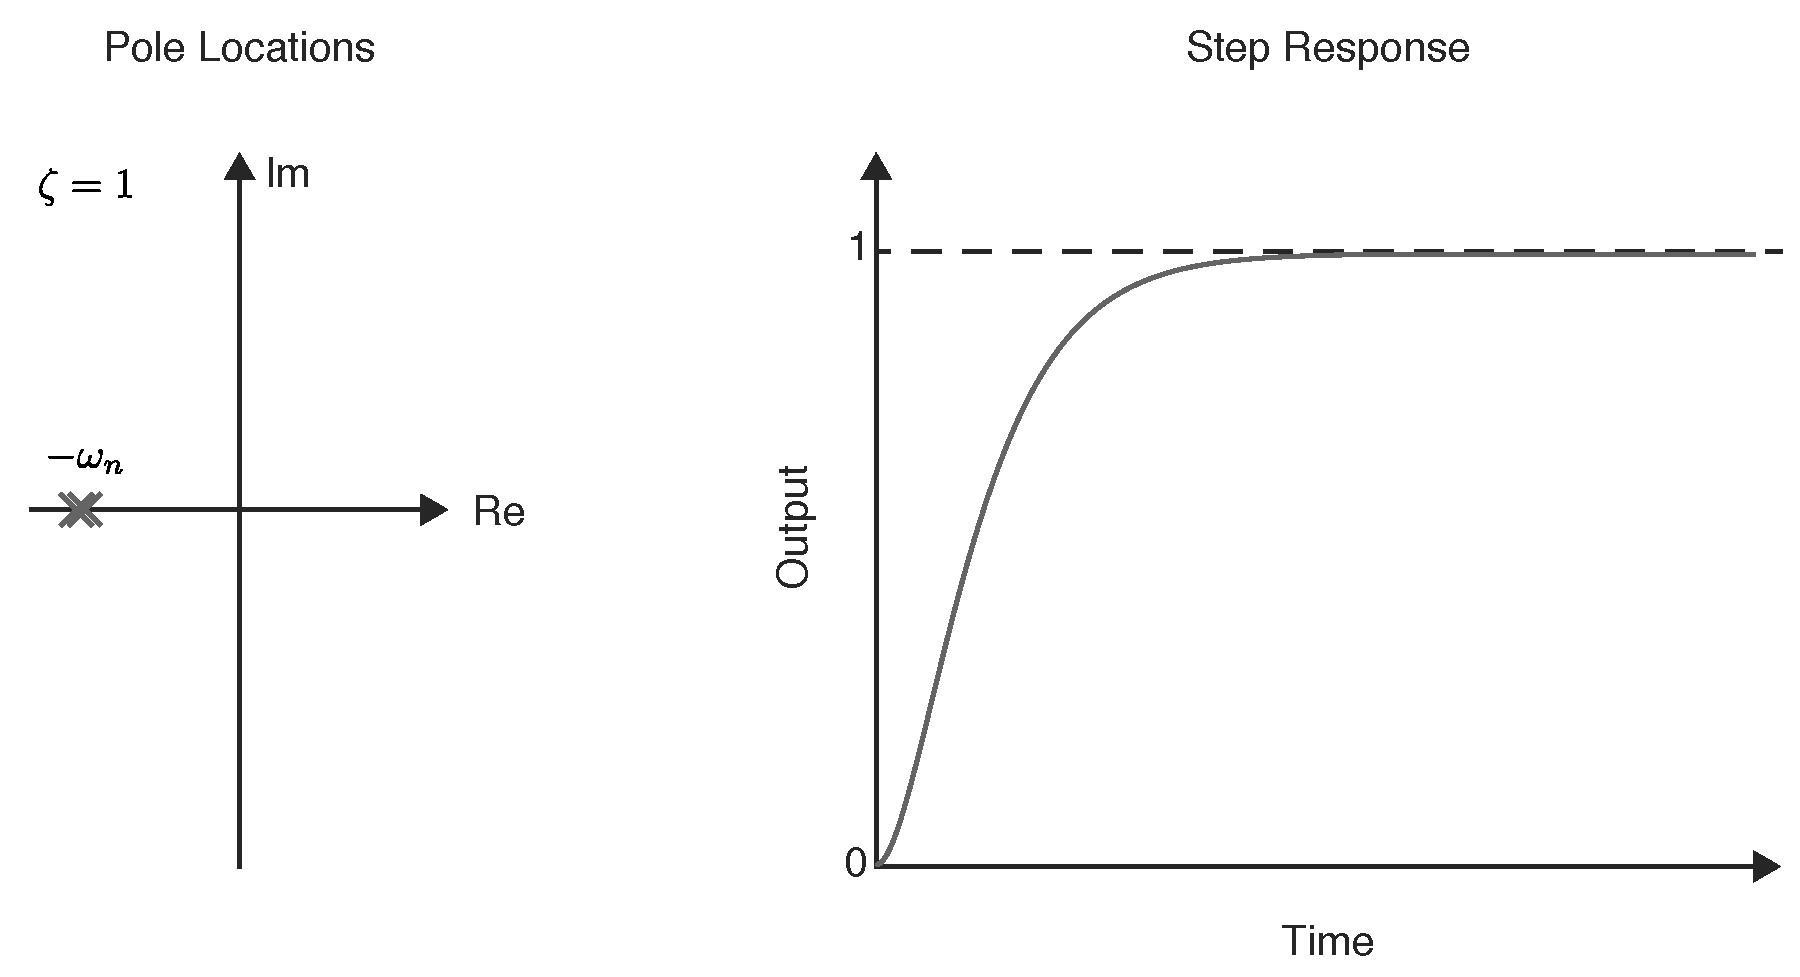
\includegraphics[width=0.75\textwidth]{critical}
    \end{center}
  \end{minipage}
  
  \textbf{Case 3:} When $\zeta > 1$, the system becomes over damped and there exist 
  two real roots
 	%
	\begin{align*}
		p_1 &= - \zeta \omega_n + \omega_n \sqrt{\zeta^2 - 1} > - \omega_n 
		\\
		p_2 &= - \zeta \omega_n - \omega_n \sqrt{\zeta^2 - 1} < - \omega_n 
	\end{align*}
%
$G(s)$ can be written in terms of $s_1$ and $s_2$ 
%
\begin{align*}
	G(s) = \frac{p_1 p_2}{(s+p_1) (s+p_2)}
\end{align*}
%
where it is easy to see that $p_1 p_2 = \omega_n^2$. Finally, we can compute the step-response as
%
\begin{align*}
 Y(s) &= G(s) U(s) = \frac{p_1 p_2}{s (s-p_1) (s-p_2)} 
 \\
 y(t) &= 1 + \frac{p_2}{p_1 - p_2} e^{p_1 t} - \frac{p_1}{p_1 - p_2} e^{p_2 t} 
 \end{align*}
 %
 Pole locations and step response when $\zeta > 1$ (over damped), is illustrated in
the Figure below

    \begin{minipage}[h]{1\linewidth}
    \begin{center}
     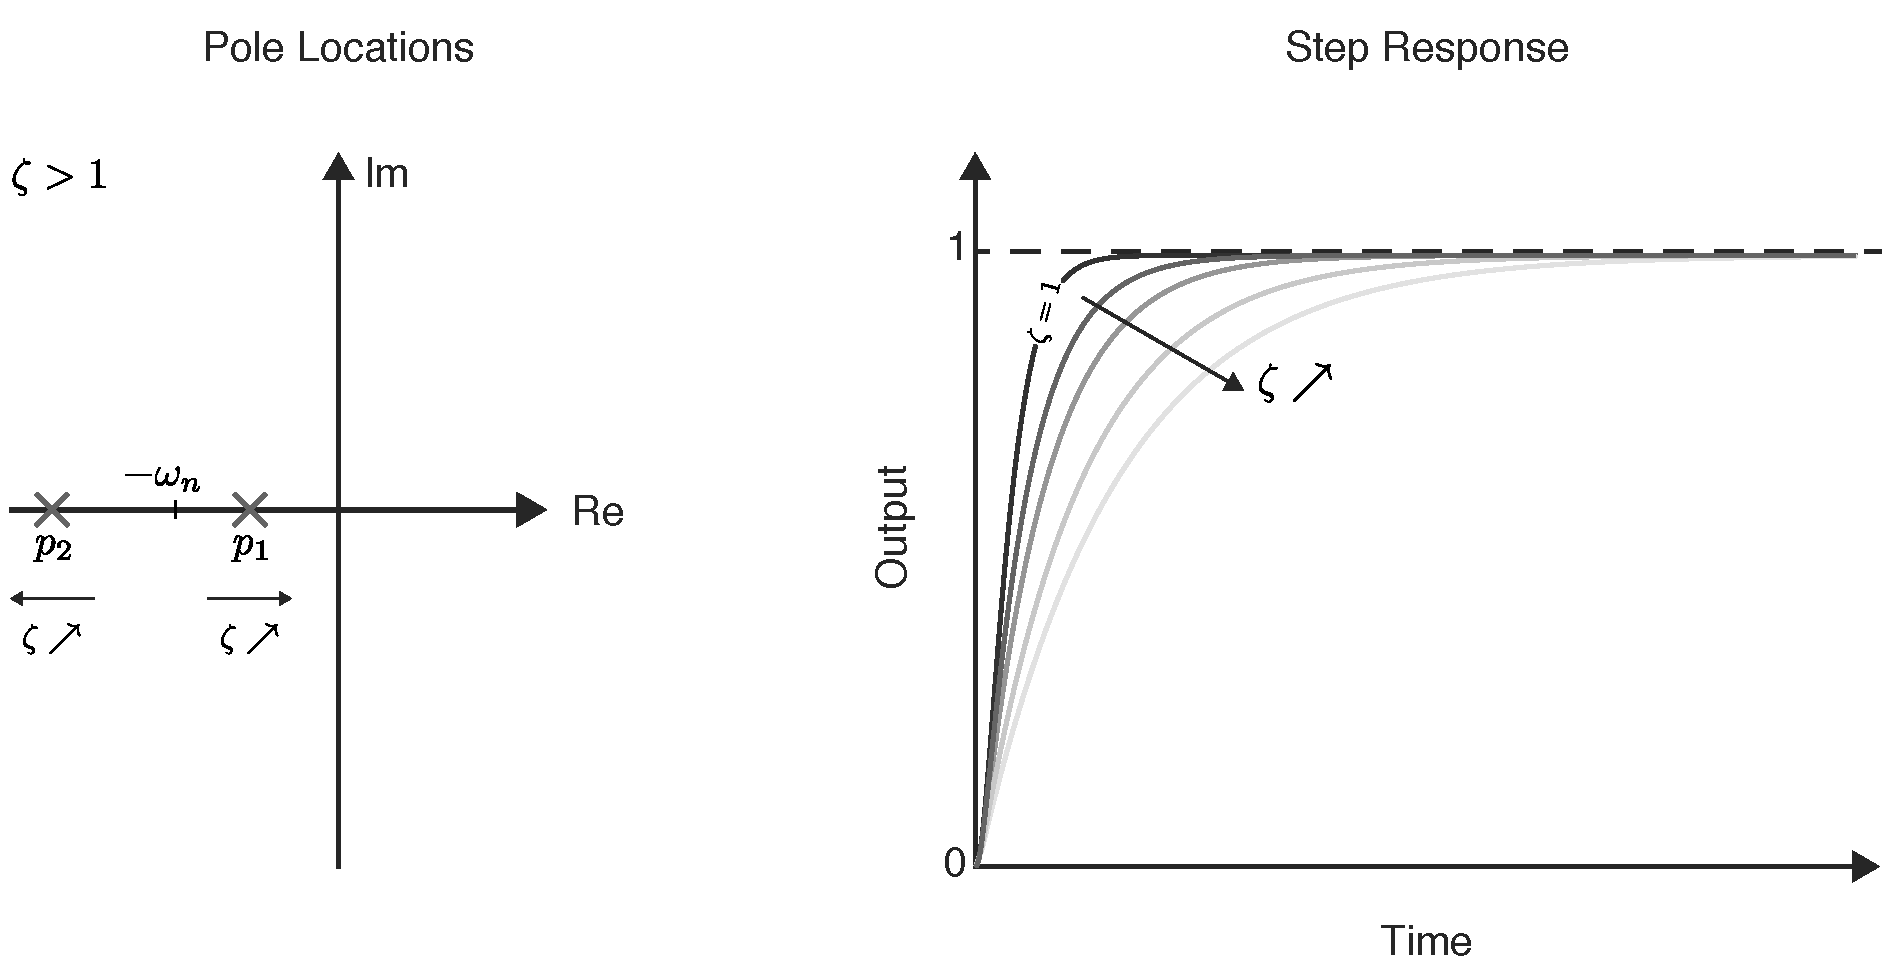
\includegraphics[width=0.9\textwidth]{over}
    \end{center}
  \end{minipage}

\textbf{Case 3:} When $0 <  \zeta < 1$, the system becomes under damped and there exist 
  two complex conjugate roots.
  %
 \begin{align*}
 p_{1,2} &= - \zeta \omega_n \pm j \omega_n \sqrt{1 - \zeta^2}
 \\
 | p_{1,2} | &= \omega_n
 \end{align*}
 %
 Let $\sigma = \zeta \omega_n$ and $\omega_d = \omega_n \sqrt{1 - \zeta^2}$ (which is called damped
 natural frequency), then we know that general solution of the ODE solution takes the form
 %
 \begin{align*}
 	y(t) = y_p(t) + C_1 e^{-\sigma t} \cos(\omega_d t) + C_2 e^{-\sigma t} \sin(\omega_d t) 
 \end{align*}
 % 
Steady-state conditions leads that $y_p(t) = 1$. Then we can compute remaining coefficients
from zero initial conditions constraints
 %
 \begin{align*}
 y(0) = 0 \quad \rightarrow \quad& C_1 = -1
 \\
 \dot{y}(0) = 0 \quad \rightarrow \quad&
\frac{d}{dt} \left[ e^{-\sigma t} [ -\cos(\omega_d t) + C_2  \sin(\omega_d t) ] \right]|_{t = 0} = 0
\\
& \left[ -\sigma e^{-\sigma t} [ -\cos(\omega_d t) + C_2  \sin(\omega_d t) ] 
+ e^{-\sigma t} [ \omega_d  \sin(\omega_d t) + C_2  \omega_d \cos(\omega_d t) ]  \right] |_{t = 0} = 0
\\
&\left[ \sigma  + C_2  \omega_d  \right] = 0
\\
&C_2 = -\frac{\sigma}{\omega_d} = -\frac{\zeta}{\sqrt{1 - \zeta^2}}
 \end{align*} 
 %
 Finally output, $y(t)$, takes the form
 %
  \begin{align*}
  y(t) = 1 - e^{-\sigma t} \left[ \cos(\omega_d t) + \frac{\zeta}{\sqrt{1 - \zeta^2}} \sin(\omega_d t) \right]
  \end{align*}
%
If we combine $\cos$ and $\sin$  terms into a single $\sin$ with phase shift we obtain
%
 %
  \begin{align*}
    y(t) &= 1 - \frac{e^{-\sigma t}}{ \sqrt{1 - \zeta^2} } \left[ \sqrt{1 - \zeta^2} \cos(\omega_d t) + \zeta \sin(\omega_d t) \right]
    \\
    \\
&= 1 - \frac{e^{- \zeta \omega_n t}}{ \sqrt{1 - \zeta^2} } \sin(\omega_d t + \phi) \quad t \geq 0
  \end{align*}
  %
  where
  %
 \begin{align*}
   \sin(\omega_d t + \phi) &=   \sin( \phi)  \cos(\omega_d t) +   \cos( \phi)   \sin(\omega_d t) 
   \\
   \cos( \phi) &= \zeta 
   \\
   \sin( \phi) &= \sqrt{1 - \zeta^2} 
   \\
   \tan( \phi) &= \frac{\sqrt{1 - \zeta^2} }{\zeta} 
\end{align*}
   %
 Pole locations and step response when $\zeta > 1$ (under damped), is illustrated in
the Figure below

    \begin{minipage}[h]{1\linewidth}
    \begin{center}
     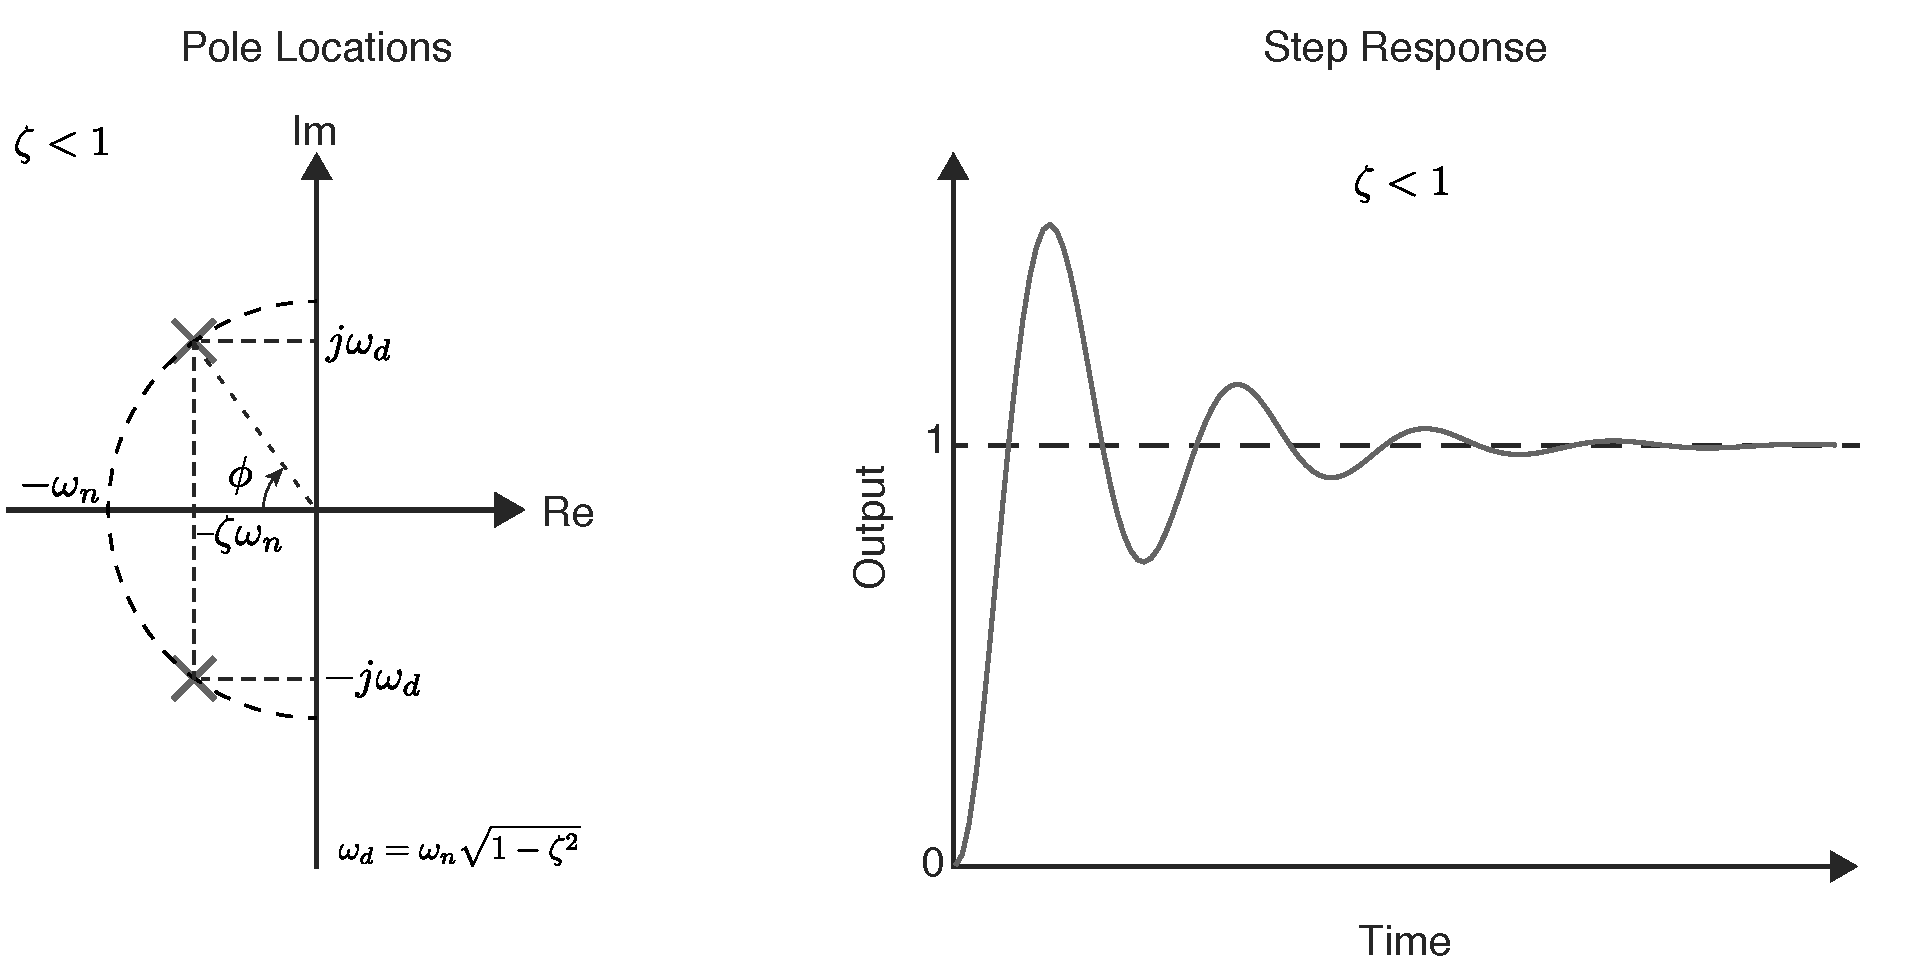
\includegraphics[width=0.9\textwidth]{under}
    \end{center}
  \end{minipage}
  
%
\subsection{Transient Response Characteristics for Underdamped Second Order Systems in Standard Form}

Important transient characteristics and performance metrics for $2^{nd}$ order underdamped systems are 
illustrated in the Figure below.

    \begin{minipage}[h]{1\linewidth}
    \begin{center}
     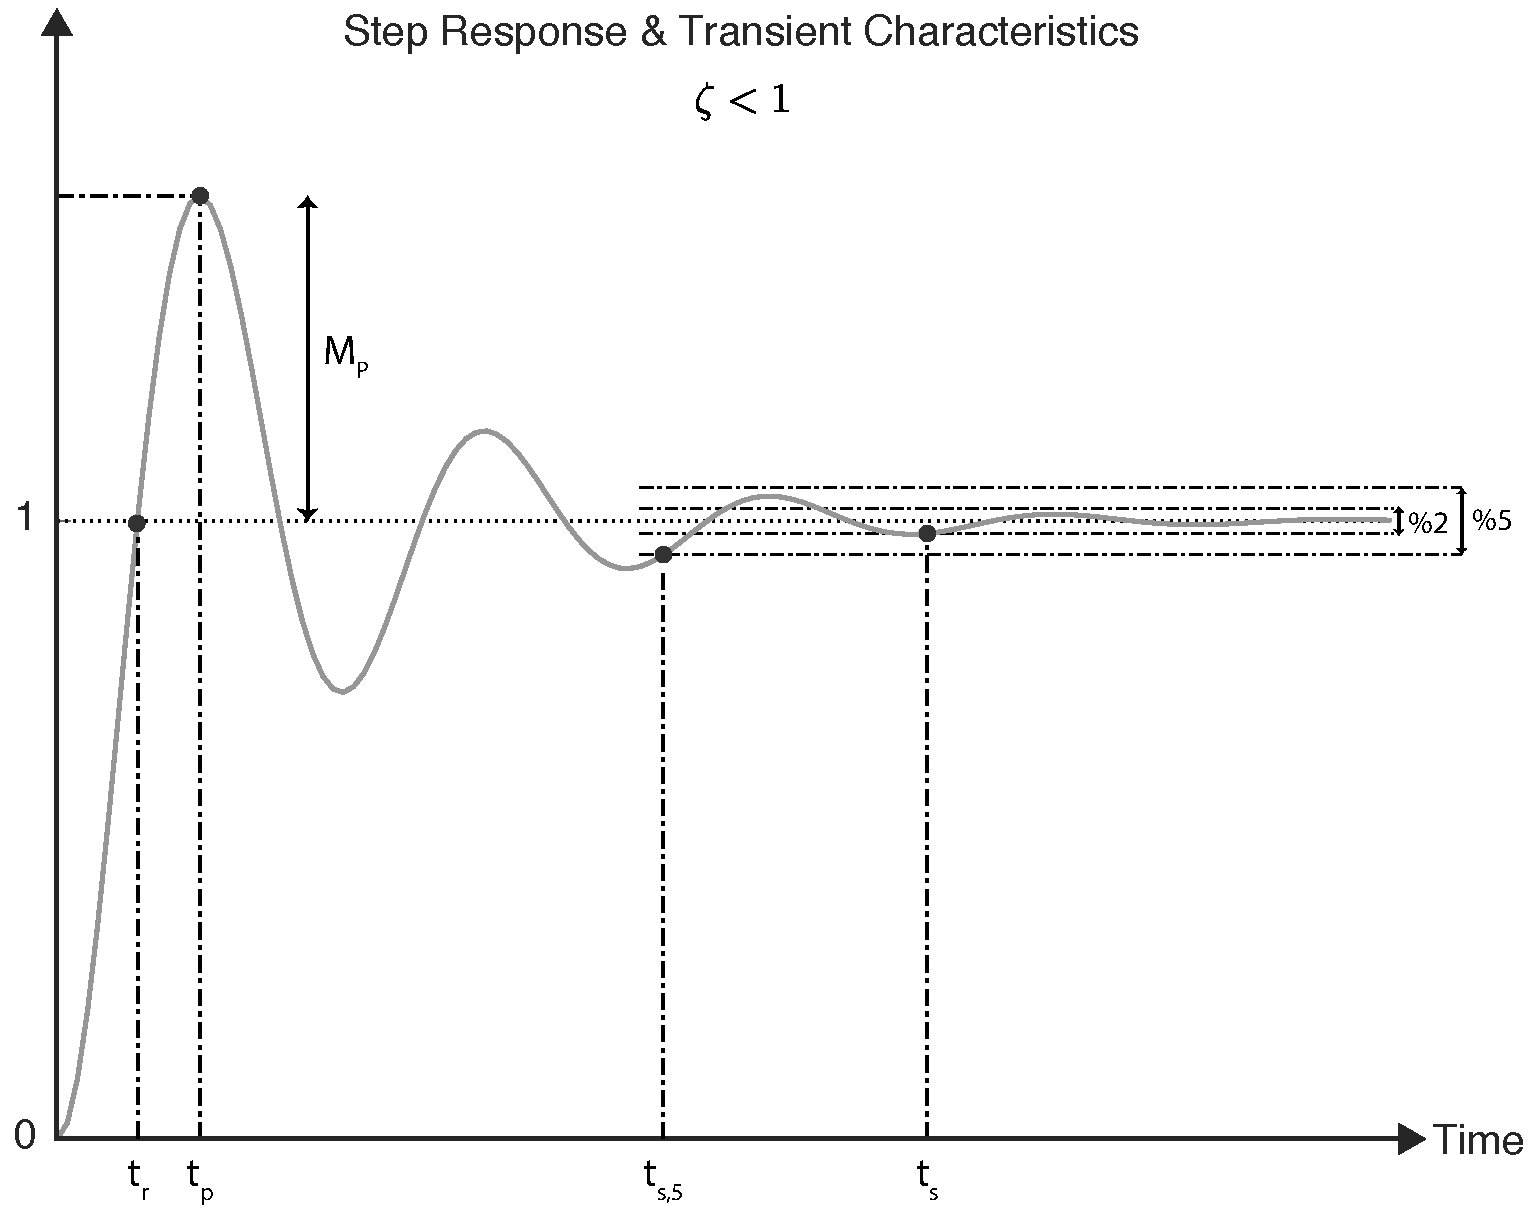
\includegraphics[width=0.8\textwidth]{transient}
    \end{center}
  \end{minipage}
  
\textbf{Rise Time ($tr$):}  The first time instant the response intersects the $y =1$ line.
%
 \begin{align*}
 y(t_r) &= 1
 \\
 1 &= 1 - \frac{e^{- \zeta \omega_n t_r}}{ \sqrt{1 - \zeta^2} } \sin(\omega_d t_r + \phi) 
 \\
 \pi &= \omega_d t_r + \phi
 \\
 t_r &= \frac{\pi - \phi}{\omega_d}
\end{align*}
  
  \textbf{Peak Time ($t_p$):}  The first time instant the response makes a peak 
  %
 \begin{align*}
& \left[  \frac{d y}{dt} \right]_{t_p} = 0
 \\
& \frac{d }{dt} \left[ - \frac{e^{-\zeta \omega_n t}}{ \sqrt{1 - \zeta^2} } \left[ \sqrt{1 - \zeta^2} \cos(\omega_d t) + \zeta \sin(\omega_d t) 
\right] \right]_{t_p} = 0
\\
& \left[ 
 \zeta \omega_n e^{-\zeta \omega_n t} \left[ \sqrt{1 - \zeta^2} \cos(\omega_d t) + \zeta \sin(\omega_d t) \right] -
e^{-\zeta \omega_n t} \left[ - \omega_d \sqrt{1 - \zeta^2} \sin(\omega_d t) + \zeta \omega_d \cos(\omega_d t) \right] 
\right]_{t_p} = 0
\\
& \left[ 
\left[  \zeta  \sqrt{1 - \zeta^2} \cos(\omega_d t) + \zeta^2 \sin(\omega_d t) \right] -
\left[ - (1 - \zeta^2) \sin(\omega_d t) + \zeta \sqrt{1 - \zeta^2} \cos(\omega_d t) \right] 
\right]_{t_p} = 0
\\
& \left[ 
 \left[  \zeta^2 \sin(\omega_d t) + (1 - \zeta^2) \sin(\omega_d t)  \right] 
\right]_{t_p} = 0
\\
&\sin(\omega_d t_{t_p})  = 0
\\
&t_p = \frac{\pi}{\omega_d}
\end{align*}
  
\textbf{Maximum Overshoot ($M_p$):}  The maximum amount by which the response exceeds the value $1$.
 %
\begin{align*}
	M_p &= y(t_p) - 1
	\\
	&= \left[1 - \frac{e^{-\zeta \omega_n t}}{ \sqrt{1 - \zeta^2} } \left[ \sqrt{1 - \zeta^2} \cos(\omega_d t) + \zeta \sin(\omega_d t) 
\right] \right]_{t_p} - 1
\\
&= \left[ \frac{e^{-\zeta \omega_n \frac{\pi}{\omega_d}}}{ \sqrt{1 - \zeta^2} } \sqrt{1 - \zeta^2} (-1) \right] 
\\
M_p &= e^{-\pi  \frac{\zeta}{\ \sqrt{1 - \zeta^2}}} = e^{\frac{-\pi}{\tan \phi}} 
\end{align*}

Maximum Percentage Overshoot ($MP_p$) is simply calculated as $MP_p =
M_p \, 100$.

\textbf{Settling Time ($t_s$):}  The earliest time instant such that
$|y(t) - 1| \leq 0.02 s$ or ($|y(t) - 1| \leq 0.05 s$) for all $t \geq
t_s$.Actual, settling time is very difficult to compute analytically (not
so hard with numerical simulations). Thus we use following
approximations.
%
\begin{align*}
  t_{s,5} &=\frac{3}{\zeta \omega_n} \quad \%5 
\\ 
  t_{s,2} &=\frac{4}{\zeta \omega_n} \quad \%2
\end{align*} 

% Since, $ | \sin(\omega_d t + \phi) | \leq 1$, we have the following
% relations
% %
% \begin{align*}
%  y(t) &\leq 1 + \frac{e^{-\zeta \omega_n t}}{\sqrt{1 - \zeta^2}} =
%   y_{eu}(t)
% \\
%  y(t) &\geq 1 - \frac{e^{-\zeta \omega_n t}}{\sqrt{1 - \zeta^2}} =
%   y_{el}(t)
% \end{align*}
% %
% where $ y_{eu}(t)$ and $y_{el}(t)$ are called the envelopes of the
% response. These envelopes are illustrated in Figure below. 
% %
%     \begin{minipage}[h]{1\linewidth}
%     \begin{center}
%      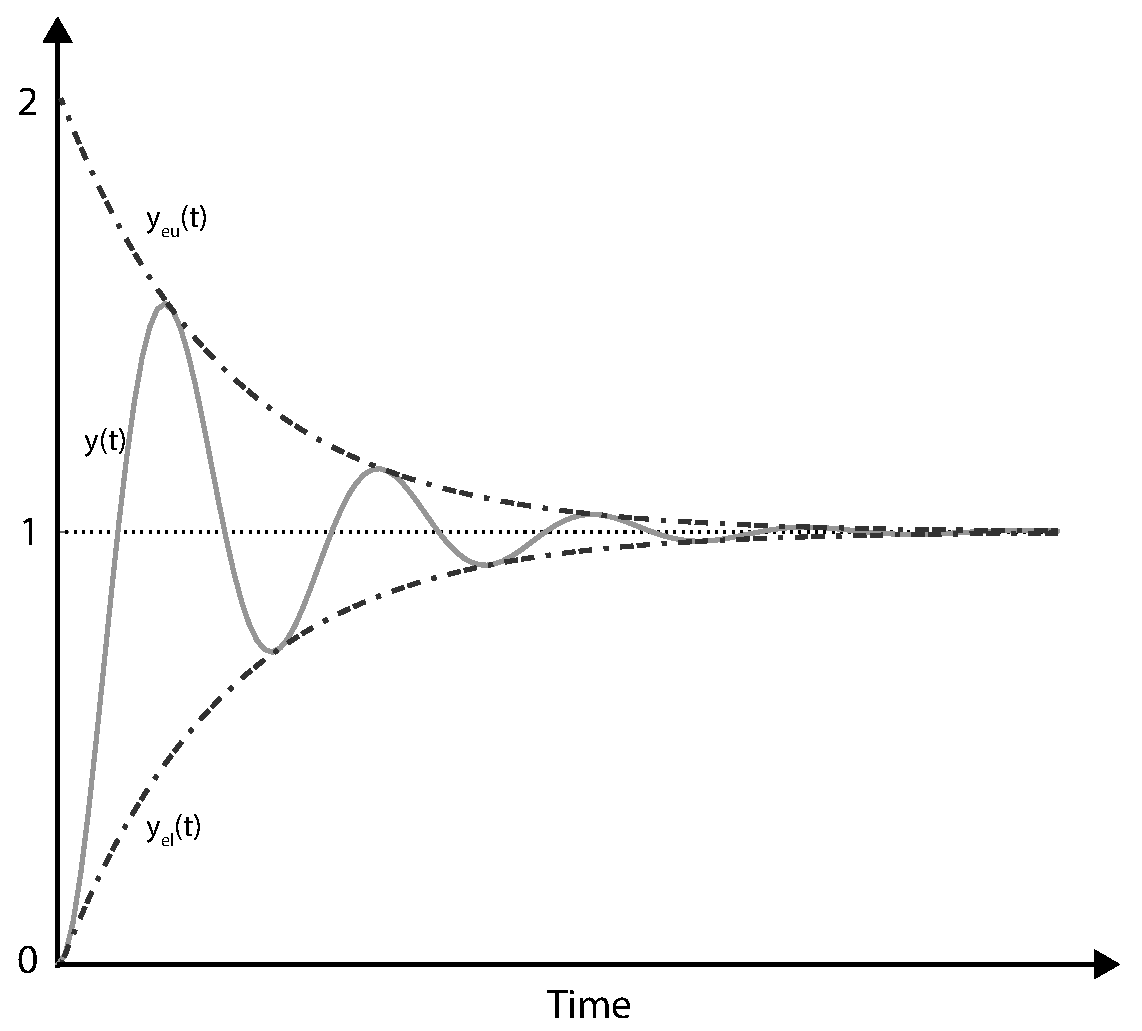
\includegraphics[width=0.9\textwidth]{envelopes}
%     \end{center}
%   \end{minipage}

\textbf{Example 1:} 

In this problem, we perform four different pole
re-location cases. During re-locations we keep some parameters
constant. Specifically
%
\begin{enumerate}
\item $p_1$ moved to a new location $p_2$ by keeping $\zeta$ (and
  $\phi$) constant.
\item $p_1$ moved to a new location $p_2$ by keeping $\omega_d$
  constant.
\item $p_1$ moved to a new location $p_2$ by keeping $\omega_n$
  constant.
\item $p_1$ moved to a new location $p_2$ by keeping $\sigma = \zeta \omega_n$
  constant.
\end{enumerate}

For each four cases, explain what happens rise time, peak time,
maximum overshoot, and settling time.

    \begin{minipage}[h]{1\linewidth}
    \begin{center}
     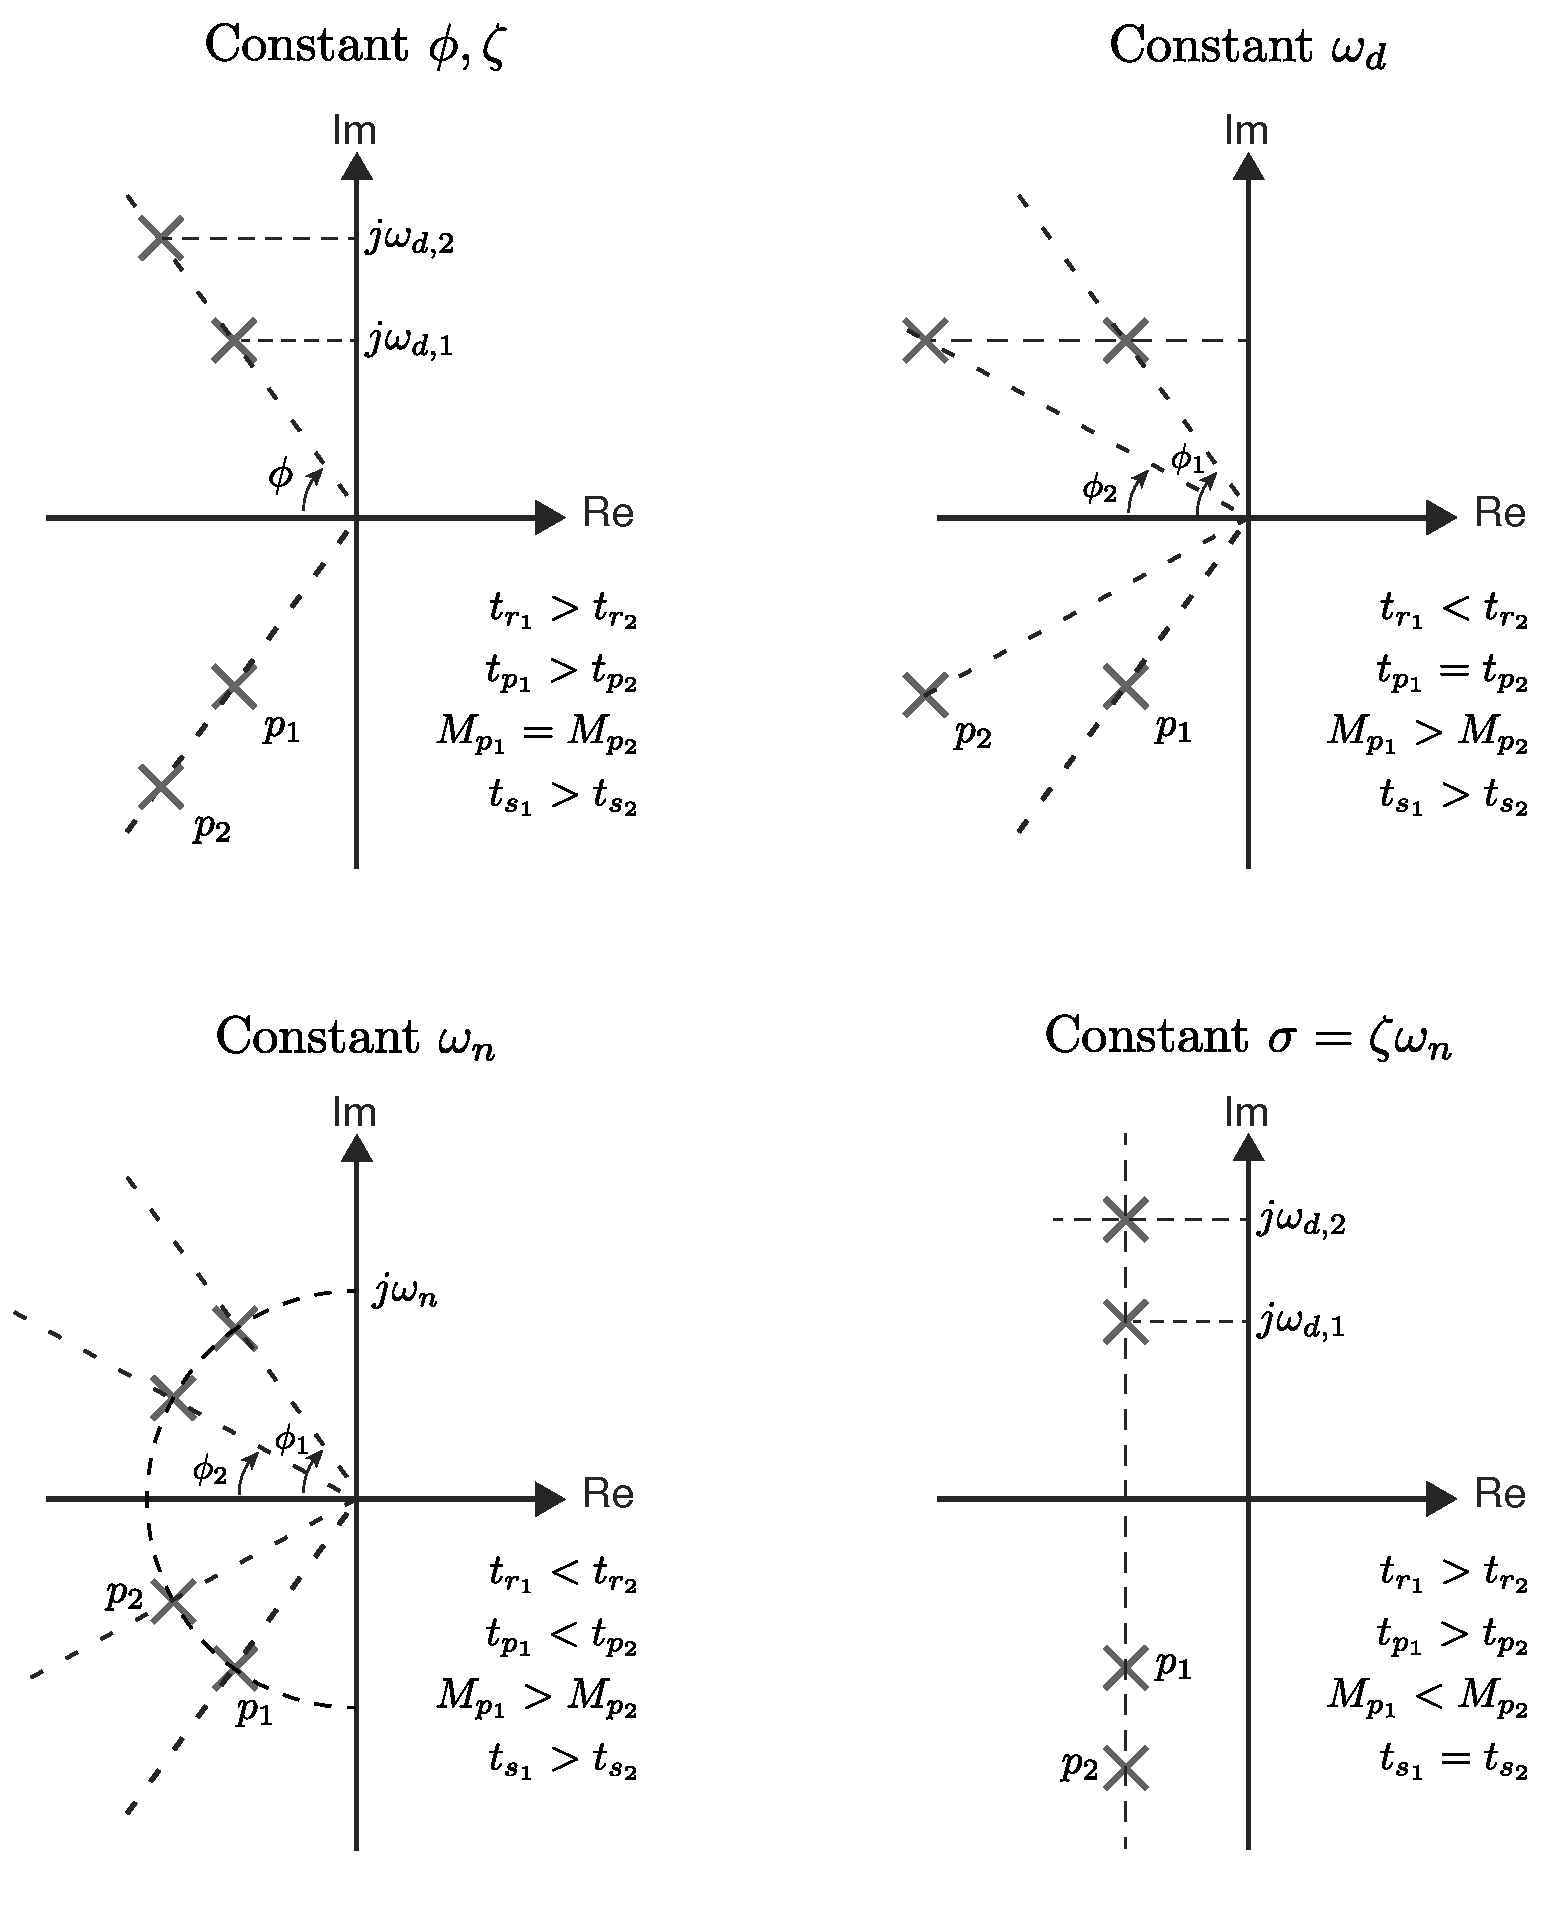
\includegraphics[width=0.83\textwidth]{ex}
    \end{center}
  \end{minipage}

\textbf{Example 2:} Consider the following closed-loop system

     \begin{minipage}[h]{1\linewidth}
    \begin{center}
     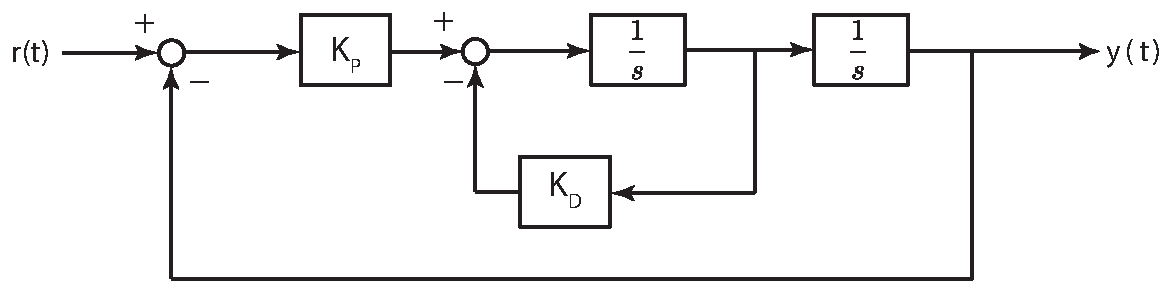
\includegraphics[width=0.8\textwidth]{example}
    \end{center}
  \end{minipage}

Design $K_P$ and $K_D$ gains such that, maximum percent overshoot is less than $\%4.32$,
and settling time ($\%2$) is less than $1$ s.

\textbf{Solution:} Lets compute the closed-loop transfer function. In order to do that, first derive the transfer
function from $E(s)$ to $Y(s)$ which is called feed-forward transfer function.
%
\begin{align*}
 \frac{Y(s)}{E(s)} = K_P \left[ \frac{1/s}{1 + K_D/s} \right] \frac{1}{s} = \frac{K_P}{s (s + K_D)}
\end{align*}
%
we can derive the $G(s)$ as
%
\begin{align*}
	G(s) = \frac{ \frac{K_P}{s (s + K_D)}}{1 +  \frac{K_P}{s (s + K_D)}} = \frac{K_P}{s^2 + K_D s + K_P}
\end{align*}
%
We can see that with $K_P$ and $K_D$ gains we have total control on the characteristic equation. 
Now let's analyze the performance requirements.

First requirement state that Maximum percent overshoot is less than $\%4.32$, which means that $M_P < 0.0432$.
Let's find a condition on $\zeta$ or $\phi$,
\begin{align*}
  M_P = e^{-\pi  \frac{\zeta}{\ \sqrt{1 - \zeta^2}}} = e^{-\pi / \tan \phi} &< 0.0432 \\
  -\pi / \tan \phi &< -\pi \\
  \tan \phi &< 1
\end{align*}
%
The region on $s$-plane that satisfy the $M_P$ requirement is illustrated below. 

     \begin{minipage}[h]{1\linewidth}
    \begin{center}
     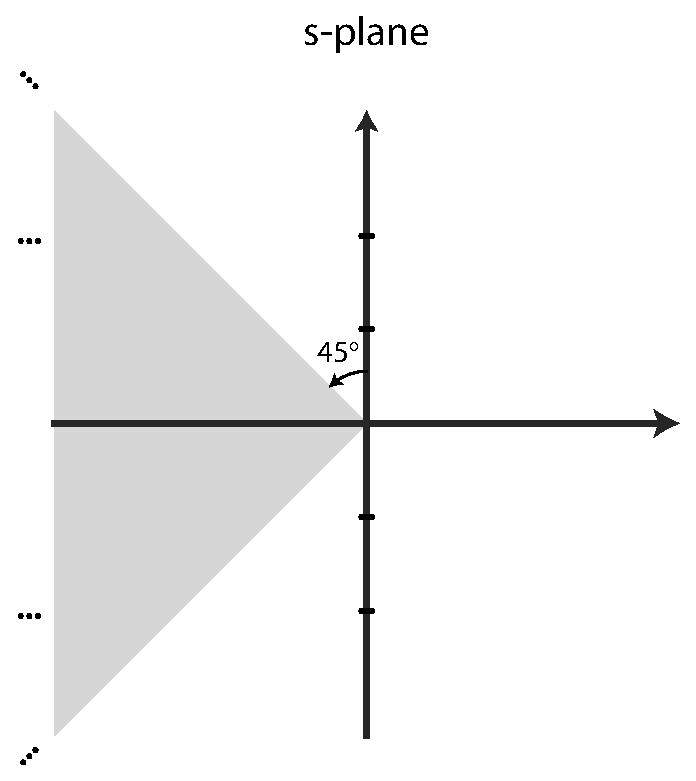
\includegraphics[width=0.35\textwidth]{damping}
    \end{center}
  \end{minipage}
  
Second requirement state that settling time ($\%2$) is less than $1$ s, which implies
%
\begin{align*}
  t_{s,2} = \frac{4}{\zeta \omega_n} = \frac{4}{\sigma} &< 1\\
  \sigma >  4
\end{align*}
%
The region on $s$-plane that satisfy the settling time requirement is illustrated below. 

     \begin{minipage}[h]{1\linewidth}
    \begin{center}
     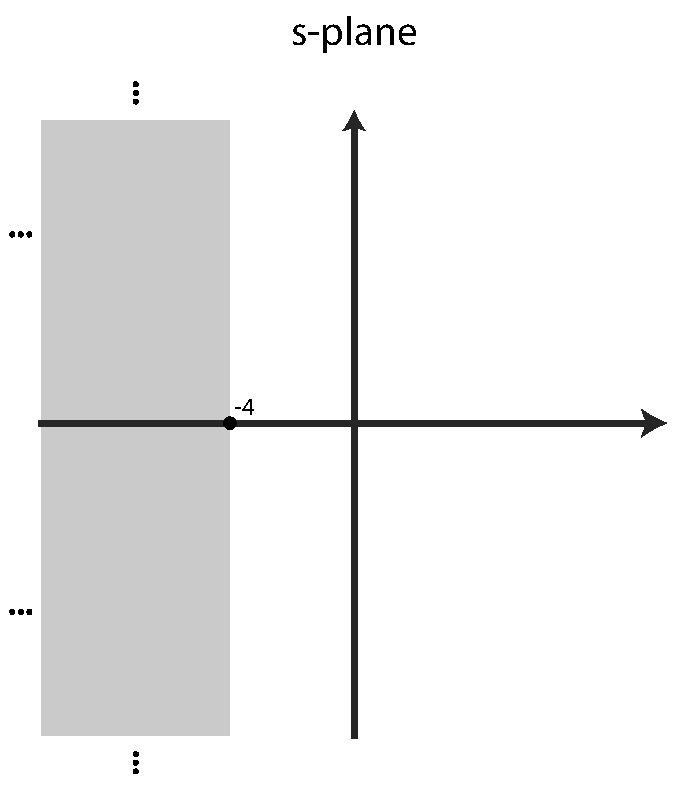
\includegraphics[width=0.35\textwidth]{settling}
    \end{center}
  \end{minipage}
  
  If we combine the requirements, we obtain the following region of possible pole locations.
  
     \begin{minipage}[h]{1\linewidth}
    \begin{center}
     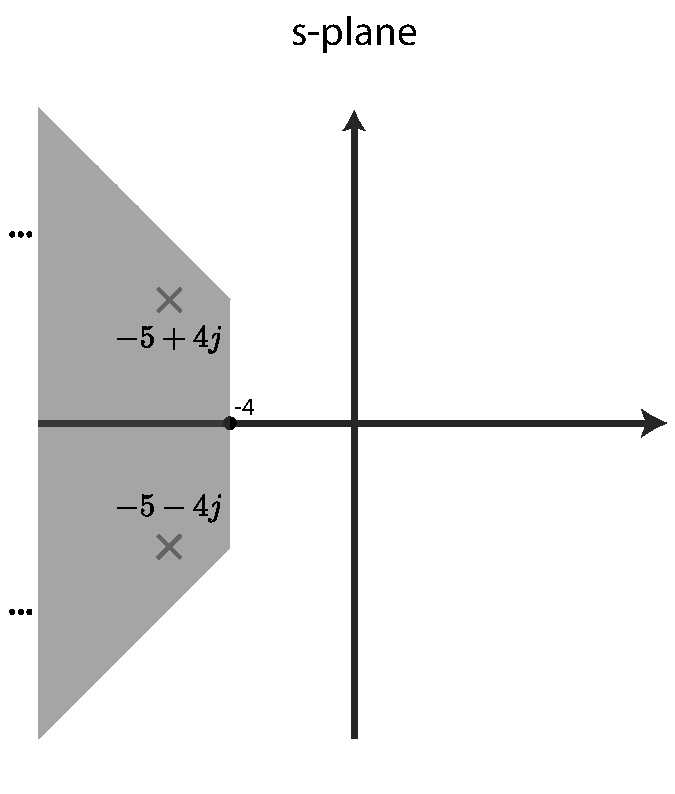
\includegraphics[width=0.4\textwidth]{result}
    \end{center}
  \end{minipage}
  
  Based on these requirements let's choose $p_{1,2} = -5 \pm 4 j$ as desired pole locations. 
  We can then compute the desired characteristic equation and then find the associated controller
  gains as
  %
  \begin{align*}
  	d^*(s) &= (s + 5 + 4 Jj (s - 5 - 4 j) = s^2 + 10 s + 41
	\\
	K_P &= 41
	\\
	K_D &= 10
  \end{align*}
  %
  If we plot the step-response, we can illustrate the performance and check if we can meet the
  requirements.
  
       \begin{minipage}[h]{1\linewidth}
    \begin{center}
     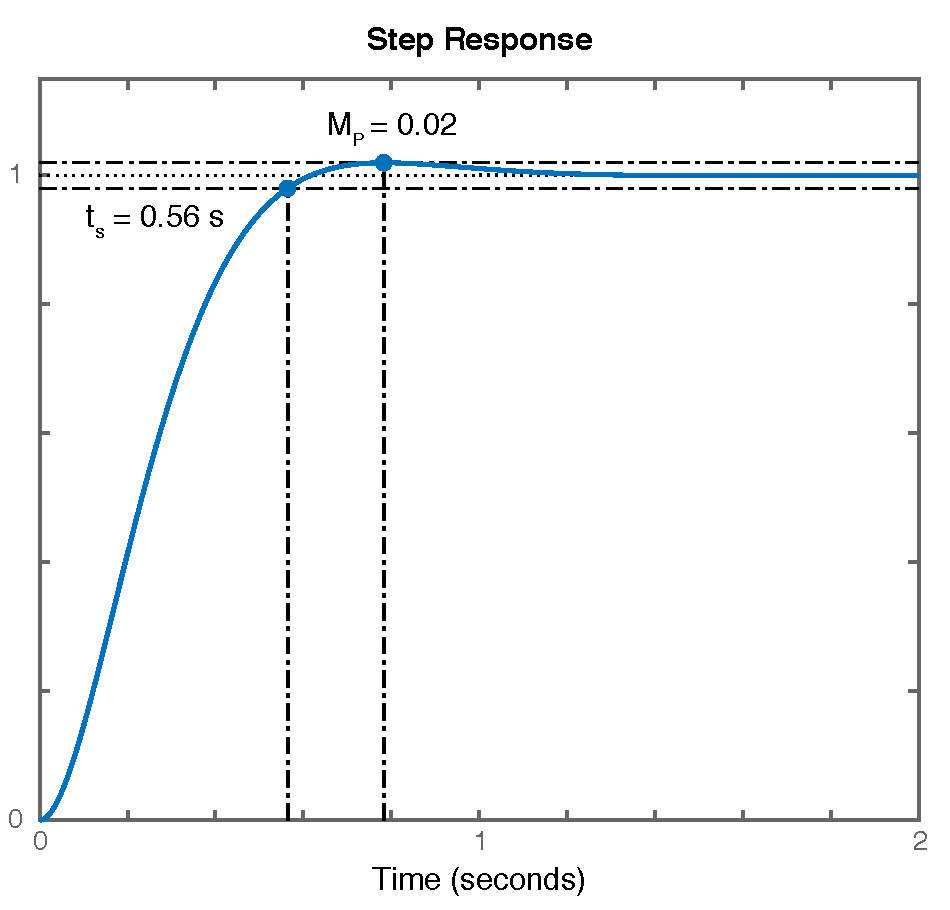
\includegraphics[width=0.45\textwidth]{stepex}
    \end{center}
  \end{minipage}
  
  \subsubsection*{Transient Specifications for Over-damped Case}

\begin{itemize}  
  \item Obviously, there is no over-shoot in over-damp case, thus $M_P = 0$.   
  \item For settling time we can use the same approximate formula by considering the dominant/slowest
  pole, i.e.
  %
  \begin{align*}
  t_{s,5} &=\frac{3}{\sigma_{min}} \quad \%5 
	\\ 
  t_{s,2} &=\frac{4}{\sigma_{min}} \quad \%2
  \end{align*}
  %
  \item Since $y(t)$ only crosses the $y = 1$ as $t \to \infty$, $t_r$ definition is not applicable for 
  over-damped case. Instead, a different rise time definition can be used (which is applicable for both
  over-damped, under-damped, critically-damped systems, as well as first order systems). $\bar{t}_r$
  is the time for $y(t)$ to go from $0.1$ to $0.9$. It is pretty hard to compute this time analytically, thus in
  general numerical and/or graphical methods are used. 
  
  Rise-time concept is illustrated in the figure below, for an example system.
  \vspace{6pt}
  
         \begin{minipage}[h]{1\linewidth}
    \begin{center}
     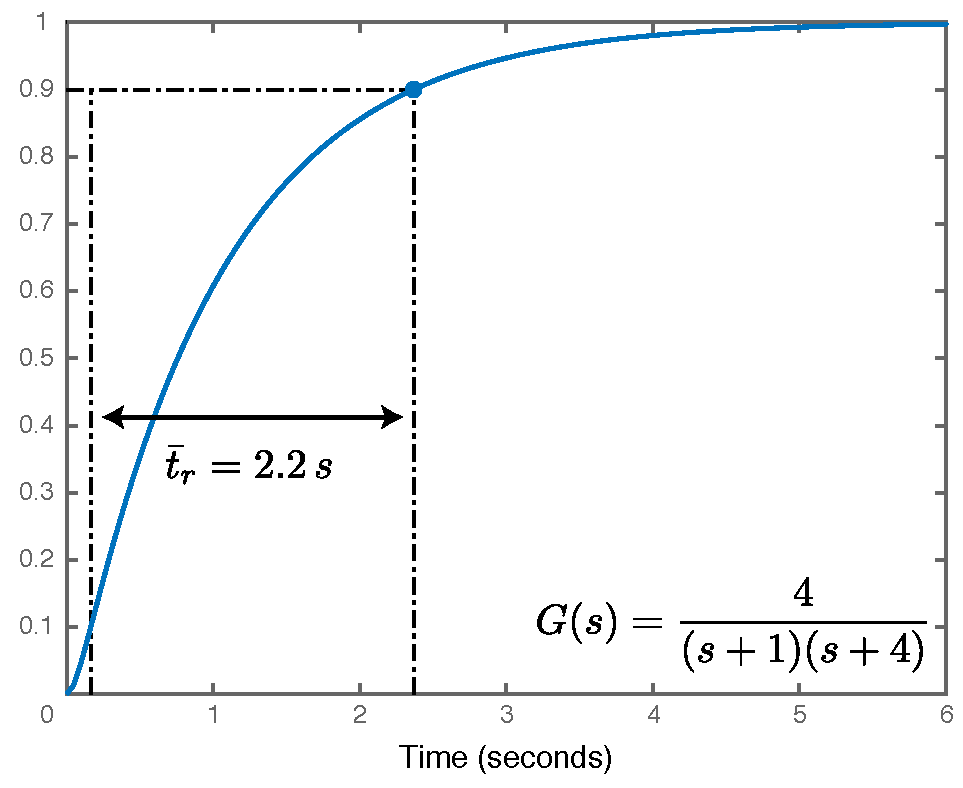
\includegraphics[width=0.45\textwidth]{rise2}
    \end{center}
  \end{minipage}
  
\end{itemize}

\section{Higher Order Systems}

In general, the poles closer to the $j \omega$ axis determine the behavior of the system. If the ``distance''
between the poles that are close to the $j \omega$ axis and other poles is high, then they dominate the
behavior and we call them dominant poles. For example, figure given below illustrates a third order system,
where we have two complex conjugate roots and one real root. In this case, the magnitude of the real pole 
is more than three times of the magnitude of the real part of the complex conjugate poles, thus the systems acts like
a second order system. 

         \begin{minipage}[h]{1\linewidth}
    \begin{center}
     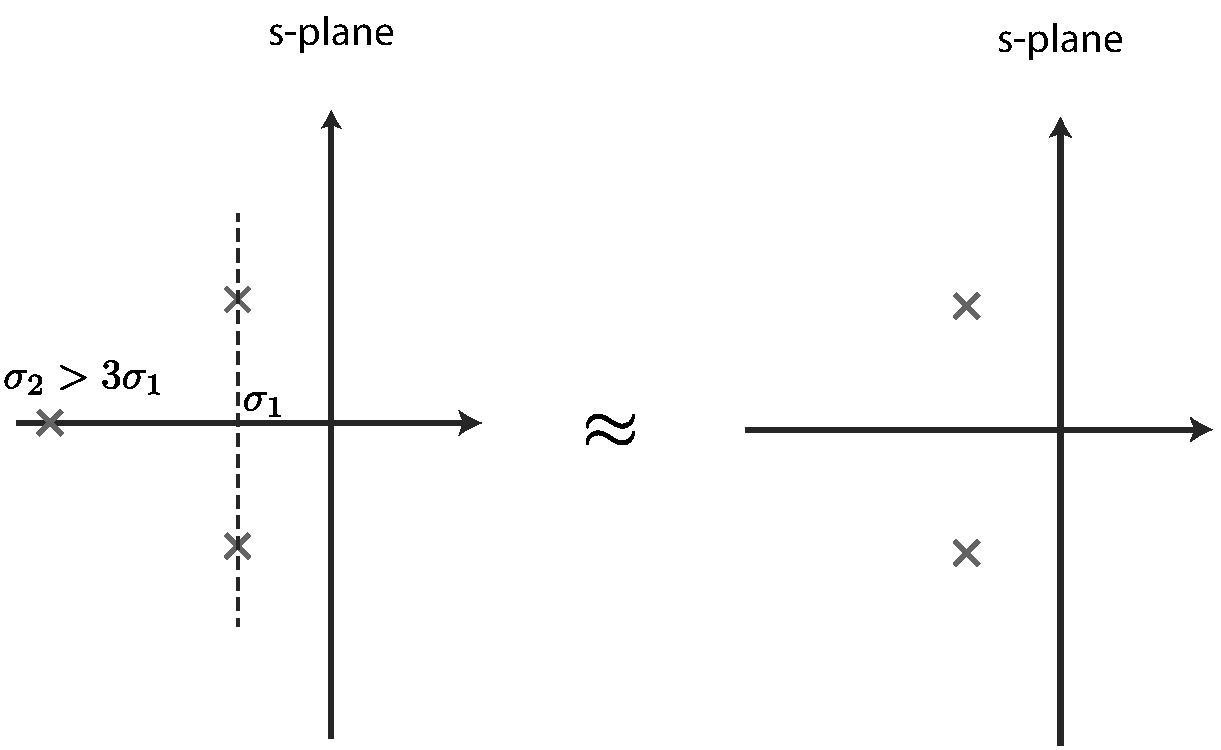
\includegraphics[width=0.6\textwidth]{third}
    \end{center}
  \end{minipage}

  
  

% **** This ENDS THE EXAMPLES. DON'T DELETE THE FOLLOWING LINE:
\end{document}